\documentclass[]{book}
\usepackage{lmodern}
\usepackage{amssymb,amsmath}
\usepackage{ifxetex,ifluatex}
\usepackage{fixltx2e} % provides \textsubscript
\ifnum 0\ifxetex 1\fi\ifluatex 1\fi=0 % if pdftex
  \usepackage[T1]{fontenc}
  \usepackage[utf8]{inputenc}
\else % if luatex or xelatex
  \ifxetex
    \usepackage{mathspec}
  \else
    \usepackage{fontspec}
  \fi
  \defaultfontfeatures{Ligatures=TeX,Scale=MatchLowercase}
\fi
% use upquote if available, for straight quotes in verbatim environments
\IfFileExists{upquote.sty}{\usepackage{upquote}}{}
% use microtype if available
\IfFileExists{microtype.sty}{%
\usepackage{microtype}
\UseMicrotypeSet[protrusion]{basicmath} % disable protrusion for tt fonts
}{}
\usepackage[margin=1in]{geometry}
\usepackage{hyperref}
\hypersetup{unicode=true,
            pdftitle={Eksploracja danych},
            pdfborder={0 0 0},
            breaklinks=true}
\urlstyle{same}  % don't use monospace font for urls
\usepackage{natbib}
\bibliographystyle{apalike}
\usepackage{longtable,booktabs}
\usepackage{graphicx,grffile}
\makeatletter
\def\maxwidth{\ifdim\Gin@nat@width>\linewidth\linewidth\else\Gin@nat@width\fi}
\def\maxheight{\ifdim\Gin@nat@height>\textheight\textheight\else\Gin@nat@height\fi}
\makeatother
% Scale images if necessary, so that they will not overflow the page
% margins by default, and it is still possible to overwrite the defaults
% using explicit options in \includegraphics[width, height, ...]{}
\setkeys{Gin}{width=\maxwidth,height=\maxheight,keepaspectratio}
\IfFileExists{parskip.sty}{%
\usepackage{parskip}
}{% else
\setlength{\parindent}{0pt}
\setlength{\parskip}{6pt plus 2pt minus 1pt}
}
\setlength{\emergencystretch}{3em}  % prevent overfull lines
\providecommand{\tightlist}{%
  \setlength{\itemsep}{0pt}\setlength{\parskip}{0pt}}
\setcounter{secnumdepth}{5}
% Redefines (sub)paragraphs to behave more like sections
\ifx\paragraph\undefined\else
\let\oldparagraph\paragraph
\renewcommand{\paragraph}[1]{\oldparagraph{#1}\mbox{}}
\fi
\ifx\subparagraph\undefined\else
\let\oldsubparagraph\subparagraph
\renewcommand{\subparagraph}[1]{\oldsubparagraph{#1}\mbox{}}
\fi

%%% Use protect on footnotes to avoid problems with footnotes in titles
\let\rmarkdownfootnote\footnote%
\def\footnote{\protect\rmarkdownfootnote}

%%% Change title format to be more compact
\usepackage{titling}

% Create subtitle command for use in maketitle
\newcommand{\subtitle}[1]{
  \posttitle{
    \begin{center}\large#1\end{center}
    }
}

\setlength{\droptitle}{-2em}

  \title{Eksploracja danych}
    \pretitle{\vspace{\droptitle}\centering\huge}
  \posttitle{\par}
    \author{true}
    \preauthor{\centering\large\emph}
  \postauthor{\par}
      \predate{\centering\large\emph}
  \postdate{\par}
    \date{2019-03-12}

%\usepackage[cp1250]{inputenc}
%\usepackage{amsmath}
\usepackage[MeX]{polski}
\usepackage{amsfonts}
\usepackage{amsthm}
\usepackage{url}
\usepackage{graphicx}
\usepackage{multicol}
\usepackage{multirow}
\usepackage{hhline}
\usepackage{array}
\usepackage{ragged2e}
\usepackage{caption}
\usepackage{tikzsymbols}
\usepackage{textcomp}
\usepackage{parskip}
\usepackage{wrapfig}
\usepackage{booktabs}
\usepackage{lscape}
\usepackage{tabu}
\usepackage{bm}
\usepackage{booktabs}
\usepackage{fontspec}


\newcommand{\zb}[1]{\buildrel #1 \over \longrightarrow}
\newcommand{\PP}{\mathrm{P}}
\newcommand{\E}{\mathrm{E}}
\newcommand{\Var}{\operatorname{Var}}
\newcommand{\Cor}{\operatorname{Cor}}
\newcommand{\Cov}{\operatorname{Cov}}
\newcommand{\Tr}{\operatorname{Tr}}
\newcommand{\row}[1]{\buildrel \text{#1} \over =}
\newcommand{\pp}{\text{p.p.}}
\newcommand{\wtt}{wtedy i tylko wtedy, gdy }
\renewcommand{\arraystretch}{1.4}

\newcommand{\btwocol}{\begin{multicols}{2}}
\newcommand{\etwocol}{\end{multicols}}

%definicje twierdzeń
\theoremstyle{plain}
\newtheorem{tw}{Twierdzenie}[section]
\newtheorem{lm}[tw]{Lemat}
\newtheorem{uw}[tw]{Uwaga}
\newtheorem{wn}[tw]{Wniosek}

\theoremstyle{definition}
\newtheorem{df}[tw]{Definicja}
\newtheorem{prz}[tw]{Przykład}
\let\proof\uuundefined
\let\endproof\uuundefined
\newenvironment{proof}[1][Dowód]{\textbf{#1} }{\ \rule{0.5em}{0.5em}}

\usepackage{makeidx}
\makeindex

\begin{document}
\maketitle

{
\setcounter{tocdepth}{1}
\tableofcontents
}
\hypertarget{wstep}{%
\chapter*{Wstęp}\label{wstep}}
\addcontentsline{toc}{chapter}{Wstęp}

\hypertarget{o-ksiazce}{%
\section*{O książce}\label{o-ksiazce}}
\addcontentsline{toc}{section}{O książce}

Niniejsza książka powstała na bazie doświadczeń autora, a głównym jej celem jest przybliżenie czytelnikowi podstaw z dziedziny \emph{Data mining} studentom kierunku \emph{Matematyka} Politechniki Lubelskiej. Będzie łączyć w sobie zarówno treści teoretyczne związane z przedstawianymi etapami eksploracji danych i budową modeli, jak i praktyczne wskazówki dotczące budowy modeli w środowisku \textbf{R} \citep{R-base}. Podane zostaną również wskazówki, jak raportować wyniki analiz i jak dokonać właściwych ilustracji wyników. Bardzo użyteczny w napisaniu książki były pakiety programu R: \textbf{bookdown} \citep{R-bookdown}, \textbf{knitr} \citep{R-knitr} oraz pakiet \textbf{rmarkdown} \citep{R-rmarkdown}.

\hypertarget{zakres-przedmiotu}{%
\section*{Zakres przedmiotu}\label{zakres-przedmiotu}}
\addcontentsline{toc}{section}{Zakres przedmiotu}

Przedmiot \emph{Eksploracja danych} będzie obejmował swoim zakresem eksplorację i wizualizację danych oraz uczenie maszynowe. Eksploracja danych ma na celu pozyskiwanie i systematyzację wiedzy pochodzącej z danych. Odbywa się ona głównie przy użyciu technik statystycznych, rachunku prawdopodobieństwa i metod z zakresu baz danych. Natomiast uczenie maszynowe, to gałąź nauki (obejmuje nie tylko statystykę, choć to na niej się głównie opiera) dotyczącej budowy modeli zdolnych do rozpoznawania wzorców, przewidywania wartości i klasyfikacji obiektów. Data mining to szybko rosnaca grupa metod analizy danych rozwijana nie tylko przez statystyków ale również przez biologów, genetyków, cybernetyków, informatyków, ekonomistów, osoby pracujace nad rozpoznawaniem obrazów i wiele innych grup zawodowych. W dzisiejszych czasch trudno sobie wyobrazić życie bez sztucznej inteligencji. Towarzyszy ona nam w codziennym, życiu kiedy korzystamy z telefonów komórkowych, wyszukiwarek internetowych, robotów sprzątających, automatycznych samochodów, nawigacji czy gier komputerowych. Lista ta jest niepełna i stale się wydłuża.

href=``\url{https://twitter.com/i/status/1091069356367200256}''\textgreater{}January 31, 2019

\hypertarget{zakres-technik-stosowanych-w-data-mining}{%
\section*{Zakres technik stosowanych w data mining}\label{zakres-technik-stosowanych-w-data-mining}}
\addcontentsline{toc}{section}{Zakres technik stosowanych w data mining}

\begin{itemize}
\tightlist
\item
  statystyka opisowa
\item
  wielowymiarowa analiza danych
\item
  analiza szeregów czasowych
\item
  analiza danych przestrzennych
\item
  reguły asocjacji
\item
  uczenie maszynowe\footnote{ang. \emph{machine learning}}, w tym:

  \begin{itemize}
  \tightlist
  \item
    klasyfikacja
  \item
    predykcja
  \item
    analiza skupień
  \item
    \emph{text mining}
  \end{itemize}
\item
  i wiele innych
\end{itemize}

\begin{figure}
\centering
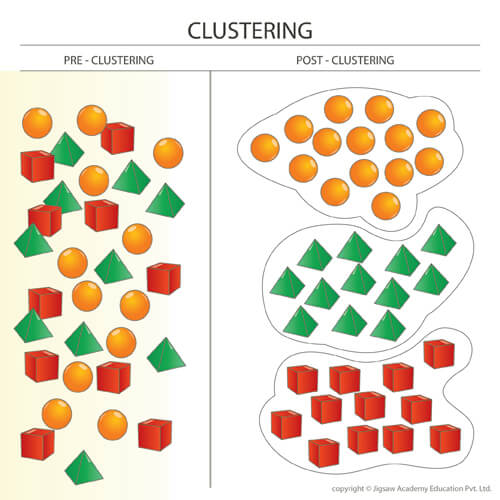
\includegraphics{images/cluster1.jpg}
\caption{\label{fig:cluster1}Przykład nienadzorowanego uczenia maszynowego.~ \emph{Źródło:}\url{https://analyticstraining.com/cluster-analysis-for-business/}}
\end{figure}

href=``\url{https://twitter.com/i/status/1097199751072690176}''\textgreater{}Ferbruary 17, 2019

\hypertarget{etapy-eksploracji-danych}{%
\section*{Etapy eksploracji danych}\label{etapy-eksploracji-danych}}
\addcontentsline{toc}{section}{Etapy eksploracji danych}

\begin{figure}
\centering
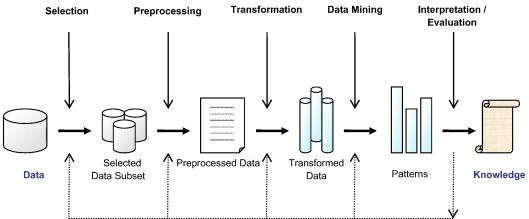
\includegraphics{images/dm_stages.jpg}
\caption{\label{fig:unnamed-chunk-2}Etapy eksploracji danych \citep{KAVAKIOTIS2017}}
\end{figure}

\begin{enumerate}
\def\labelenumi{\arabic{enumi}.}
\tightlist
\item
  Czyszczenie danych - polega na usuwaniu braków danych, usuwaniu stałych zmiennych, imputacji braków danych oraz przygotowaniu danych do dalszych analiz.
\item
  Integracja danych - łączenie danych pochodzących z różnych źródeł.
\item
  Selekcja danych - wybór z bazy tych danych, które są potrzebne do dalszych analiz.
\item
  Transformacja danych - przekształcenie i konsolidacja danych do postaci przydatnej do eksploracji.
\item
  Eksploracja danych - zastosowanie technik wymienionych wcześniej w celu odnalezienia wzorców\footnote{ang. \emph{patterns}} i zależności.
\item
  Ewaluacja modeli - ocena poprawności modeli oraz wzorców z nich uzyskanych.
\item
  Wizualizacja wyników - graficzne przedstawienie odkrytych wzorców.
\item
  Wdrażanie modeli - zastosowanie wyznaczonych wzorców.
\end{enumerate}

\hypertarget{roz1}{%
\chapter{Import danych}\label{roz1}}

Placeholder

\hypertarget{przyk1}{%
\section{Przykład}\label{przyk1}}

\hypertarget{przygotowanie-danych}{%
\chapter{Przygotowanie danych}\label{przygotowanie-danych}}

Placeholder

\hypertarget{korekta-zbioru-danych}{%
\section{Korekta zbioru danych}\label{korekta-zbioru-danych}}

\hypertarget{identyfikacja-brakow-danych}{%
\subsection{Identyfikacja braków danych}\label{identyfikacja-brakow-danych}}

\hypertarget{zastepowanie-brakow-danych}{%
\subsection{Zastępowanie braków danych}\label{zastepowanie-brakow-danych}}

\hypertarget{przyk21}{%
\section{Przykład}\label{przyk21}}

\hypertarget{podzia-metod-data-mining}{%
\chapter{Podział metod data mining}\label{podzia-metod-data-mining}}

Placeholder

\hypertarget{rodzaje-wnioskowania}{%
\section{Rodzaje wnioskowania}\label{rodzaje-wnioskowania}}

\hypertarget{dziedzina}{%
\subsection{Dziedzina}\label{dziedzina}}

\hypertarget{obserwacja}{%
\subsection{Obserwacja}\label{obserwacja}}

\hypertarget{atrybuty-obserwacji}{%
\subsection{Atrybuty obserwacji}\label{atrybuty-obserwacji}}

\hypertarget{zbior-uczacy}{%
\subsection{Zbiór uczący}\label{zbior-uczacy}}

\hypertarget{zbior-testowy}{%
\subsection{Zbiór testowy}\label{zbior-testowy}}

\hypertarget{model}{%
\subsection{Model}\label{model}}

\hypertarget{jakosc-dopasowania-modelu}{%
\subsection{Jakość dopasowania modelu}\label{jakosc-dopasowania-modelu}}

\hypertarget{modele-regresyjne}{%
\section{Modele regresyjne}\label{modele-regresyjne}}

\hypertarget{modele-klasyfikacyjne}{%
\section{Modele klasyfikacyjne}\label{modele-klasyfikacyjne}}

\hypertarget{modele-grupujace}{%
\section{Modele grupujące}\label{modele-grupujace}}

\hypertarget{drzewa-decyzyjne}{%
\chapter{Drzewa decyzyjne}\label{drzewa-decyzyjne}}

Placeholder

\hypertarget{wezy-i-gaezie}{%
\section{Węzły i gałęzie}\label{wezy-i-gaezie}}

\hypertarget{rodzaje-regu-podziau}{%
\section{Rodzaje reguł podziału}\label{rodzaje-regu-podziau}}

\hypertarget{podziay-dla-atrybutow-ze-skali-nominalnej}{%
\subsection{Podziały dla atrybutów ze skali nominalnej}\label{podziay-dla-atrybutow-ze-skali-nominalnej}}

\hypertarget{podziay-dla-atrybutow-ze-skali-ciagej}{%
\subsection{Podziały dla atrybutów ze skali ciągłej}\label{podziay-dla-atrybutow-ze-skali-ciagej}}

\hypertarget{podziay-dla-atrybutow-ze-skali-porzadkowej}{%
\subsection{Podziały dla atrybutów ze skali porządkowej}\label{podziay-dla-atrybutow-ze-skali-porzadkowej}}

\hypertarget{algorytm-budowy-drzewa}{%
\section{Algorytm budowy drzewa}\label{algorytm-budowy-drzewa}}

\hypertarget{kryteria-zatrzymania}{%
\section{Kryteria zatrzymania}\label{kryteria-zatrzymania}}

\hypertarget{reguy-podziau}{%
\section{Reguły podziału}\label{reguy-podziau}}

\hypertarget{przycinanie-drzewa-decyzyjnego}{%
\section{Przycinanie drzewa decyzyjnego}\label{przycinanie-drzewa-decyzyjnego}}

\hypertarget{przycinanie-redukujace-bad}{%
\subsection{Przycinanie redukujące błąd}\label{przycinanie-redukujace-bad}}

\hypertarget{przycinanie-minimalizujace-bad}{%
\subsection{Przycinanie minimalizujące błąd}\label{przycinanie-minimalizujace-bad}}

\hypertarget{przycinanie-ze-wzgledu-na-wspoczynnik-zozonosci-drzewa}{%
\subsection{Przycinanie ze względu na współczynnik złożoności drzewa}\label{przycinanie-ze-wzgledu-na-wspoczynnik-zozonosci-drzewa}}

\hypertarget{obsuga-brakow-danych}{%
\section{Obsługa braków danych}\label{obsuga-brakow-danych}}

\hypertarget{zalety-i-wady}{%
\section{Zalety i wady}\label{zalety-i-wady}}

\hypertarget{zalety}{%
\subsection{Zalety}\label{zalety}}

\hypertarget{wady}{%
\subsection{Wady}\label{wady}}

\hypertarget{przyk41}{%
\section{Przykład}\label{przyk41}}

\hypertarget{podzia-zbioru-na-probe-uczaca-i-testowa}{%
\subsection{Podział zbioru na próbę uczącą i testową}\label{podzia-zbioru-na-probe-uczaca-i-testowa}}

\hypertarget{budowa-drzewa}{%
\subsection{Budowa drzewa}\label{budowa-drzewa}}

\hypertarget{przycinanie-drzewa}{%
\subsection{Przycinanie drzewa}\label{przycinanie-drzewa}}

\hypertarget{ocena-dopasowania-modelu}{%
\subsection{Ocena dopasowania modelu}\label{ocena-dopasowania-modelu}}

\hypertarget{inne-algorytmy-budowy-drzew-decyzyjnych-implementowane-w-r}{%
\section{\texorpdfstring{Inne algorytmy budowy drzew decyzyjnych implementowane w \textbf{R}}{Inne algorytmy budowy drzew decyzyjnych implementowane w R}}\label{inne-algorytmy-budowy-drzew-decyzyjnych-implementowane-w-r}}

\hypertarget{przyk42}{%
\section{Przykład}\label{przyk42}}

\hypertarget{ctree}{%
\subsection{\texorpdfstring{\texttt{ctree}}{ctree}}\label{ctree}}

\hypertarget{j48}{%
\subsection{\texorpdfstring{\texttt{J48}}{J48}}\label{j48}}

\hypertarget{c50}{%
\subsection{\texorpdfstring{\texttt{C50}}{C50}}\label{c50}}

\hypertarget{pochodne-drzew-decyzyjnych}{%
\chapter{Pochodne drzew decyzyjnych}\label{pochodne-drzew-decyzyjnych}}

Placeholder

\hypertarget{bagging}{%
\section{Bagging}\label{bagging}}

\hypertarget{przyk51}{%
\subsection{Przykład}\label{przyk51}}

\hypertarget{lasy-losowe}{%
\section{Lasy losowe}\label{lasy-losowe}}

\hypertarget{przyk52}{%
\subsection{Przykład}\label{przyk52}}

\hypertarget{boosting}{%
\section{Boosting}\label{boosting}}

\bibliography{book.bib,packages.bib}


\end{document}
